
\subsubsection{5.1 Existence of Contamination-Correction Signature (H-E1)}

\begin{figure}[htbp]
\centering
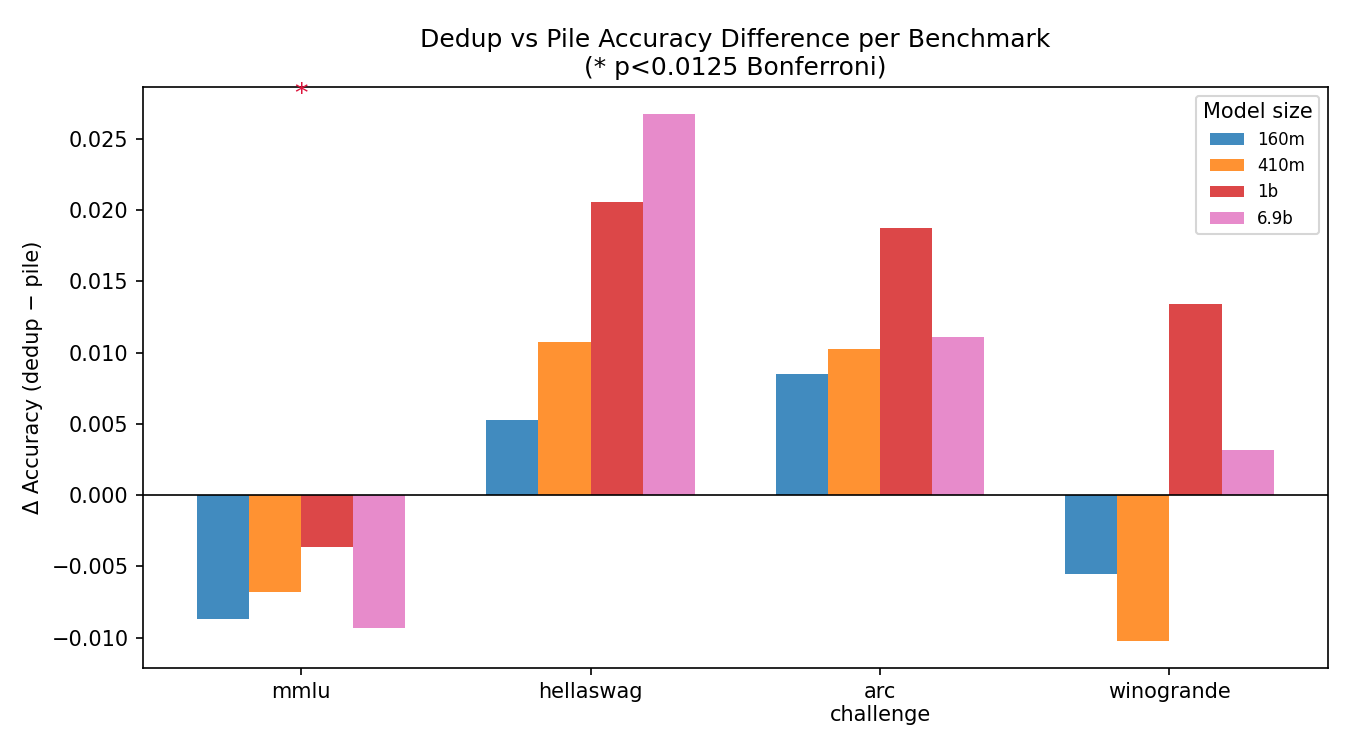
\includegraphics[width=\columnwidth]{figures/differential_bar.png}
\caption{Per-benchmark accuracy differential (dedup-Pile minus Pile) across model sizes}
\label{fig:differential_bar}
\end{figure}

\textit{Figure 1. Per-benchmark accuracy differential (dedup-Pile minus Pile) across four model sizes (160M--6.9B). MMLU consistently shows a negative differential (Pile higher); HellaSwag and ARC-Challenge show positive differentials.}

The per-benchmark accuracy differential is not uniform across benchmarks. Table 1 reports paired t-test results (n = 4 model sizes) with Bonferroni correction at alpha = 0.0125:

\textbf{Table 1. H-E1 Statistical Results: Paired t-test (n = 4 model sizes, Bonferroni alpha = 0.0125)}

\begin{table*}[htbp]
\centering
\resizebox{\dimexpr 2\columnwidth+\columnsep\relax}{!}{%
\begin{tabular}{lllll}
\toprule
Benchmark & t-statistic & p-value & Mean Delta (dedup-Pile) & Bonferroni Significant \\
\midrule
MMLU & -5.574 & 0.0114 & -0.0071 & Yes \\
HellaSwag & +3.283 & 0.0463 & +0.0159 & No \\
ARC-Challenge & +5.362 & 0.0127 & +0.0122 & No (borderline) \\
WinoGrande & +0.038 & 0.9722 & +0.0002 & No \\
\bottomrule
\end{tabular}
}
\end{table*}

MMLU is the only benchmark reaching Bonferroni-corrected significance. Its negative mean differential (-0.0071) indicates Pile-trained models score higher on MMLU than dedup-Pile models at matched token counts.

Raw accuracy values by model size and corpus are shown in Table 2:

\textbf{Table 2. Raw Accuracy Values by Model Size and Corpus}

\begin{table*}[htbp]
\centering
\resizebox{\dimexpr 2\columnwidth+\columnsep\relax}{!}{%
\begin{tabular}{llllll}
\toprule
Model & Corpus & MMLU & HellaSwag & ARC-Challenge & WinoGrande \\
\midrule
160M & Pile & 0.2619 & 0.2854 & 0.1928 & 0.5209 \\
160M & dedup-Pile & 0.2532 & 0.2907 & 0.2014 & 0.5154 \\
410M & Pile & 0.2623 & 0.3342 & 0.2133 & 0.5430 \\
410M & dedup-Pile & 0.2554 & 0.3450 & 0.2235 & 0.5328 \\
1B & Pile & 0.2515 & 0.3690 & 0.2517 & 0.5249 \\
1B & dedup-Pile & 0.2479 & 0.3896 & 0.2705 & 0.5383 \\
6.9B & Pile & 0.2716 & 0.4690 & 0.3524 & 0.6283 \\
6.9B & dedup-Pile & 0.2623 & 0.4958 & 0.3635 & 0.6314 \\
\bottomrule
\end{tabular}
}
\end{table*}

\begin{figure}[htbp]
\centering
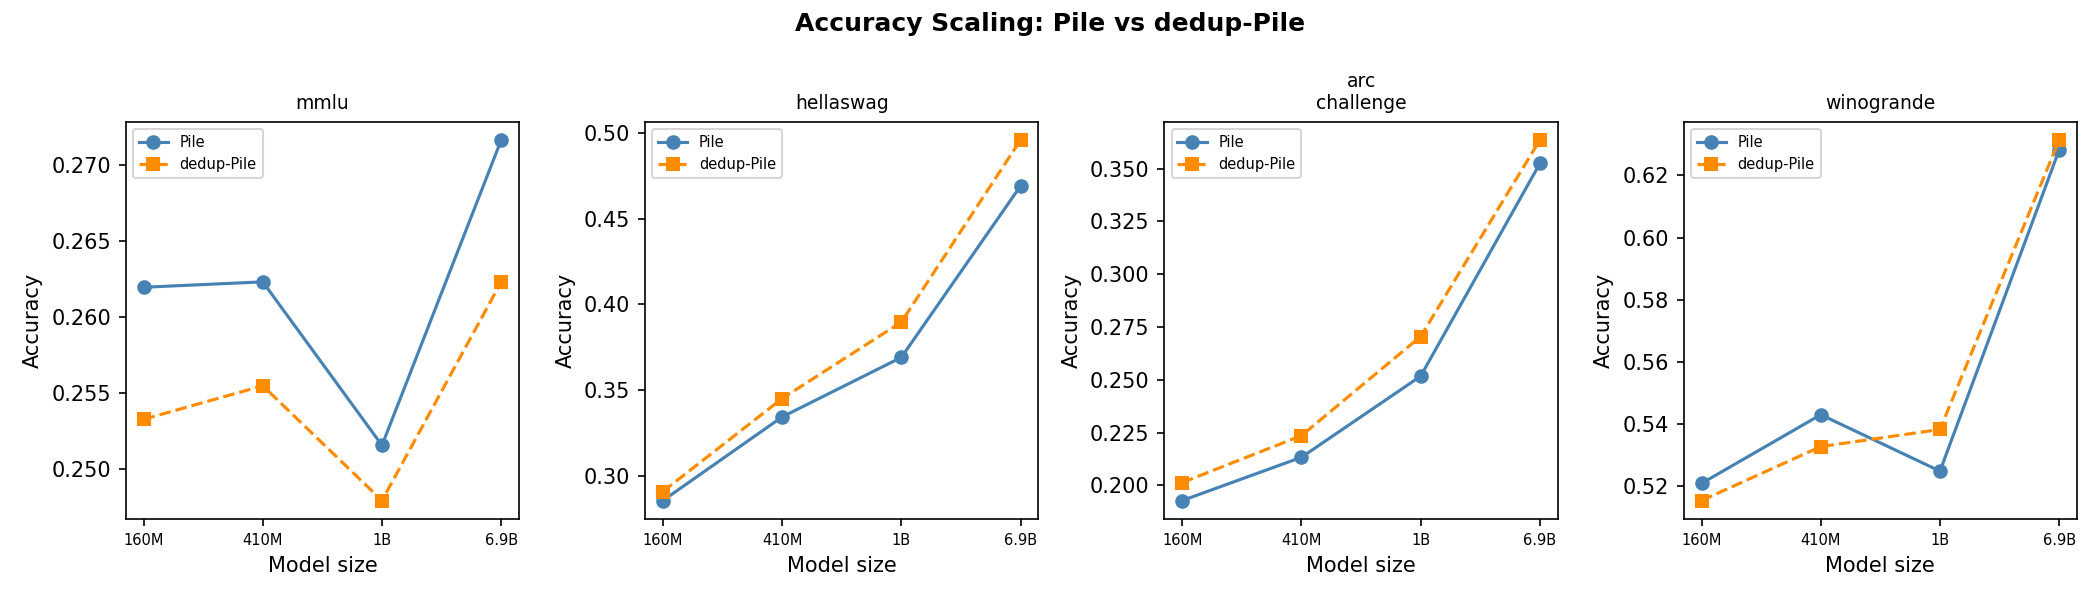
\includegraphics[width=\columnwidth]{figures/scaling_plot.png}
\caption{Scaling curves for Pile and dedup-Pile across model sizes}
\label{fig:scaling_plot}
\end{figure}

\textit{Figure 2. Benchmark accuracy scaling curves across model sizes for Pile and dedup-Pile. The MMLU lines (Pile vs dedup-Pile) diverge consistently; other benchmarks show dedup-Pile at or above Pile.}

The consistency of the MMLU differential across all four model sizes (all negative) is the basis for the significant paired t-test result. The direction is consistent with the contamination-correction hypothesis: MMLU has the second-highest estimated contamination rate (5.5\%) and shows a reduction under deduplication. However, HellaSwag, which has the highest contamination estimate (20.0\%), shows dedup-Pile higher --- a result that is discussed in Section 6.

\subsubsection{5.2 Contamination Predicts the Signature Direction (H-M3)}

\begin{figure}[htbp]
\centering
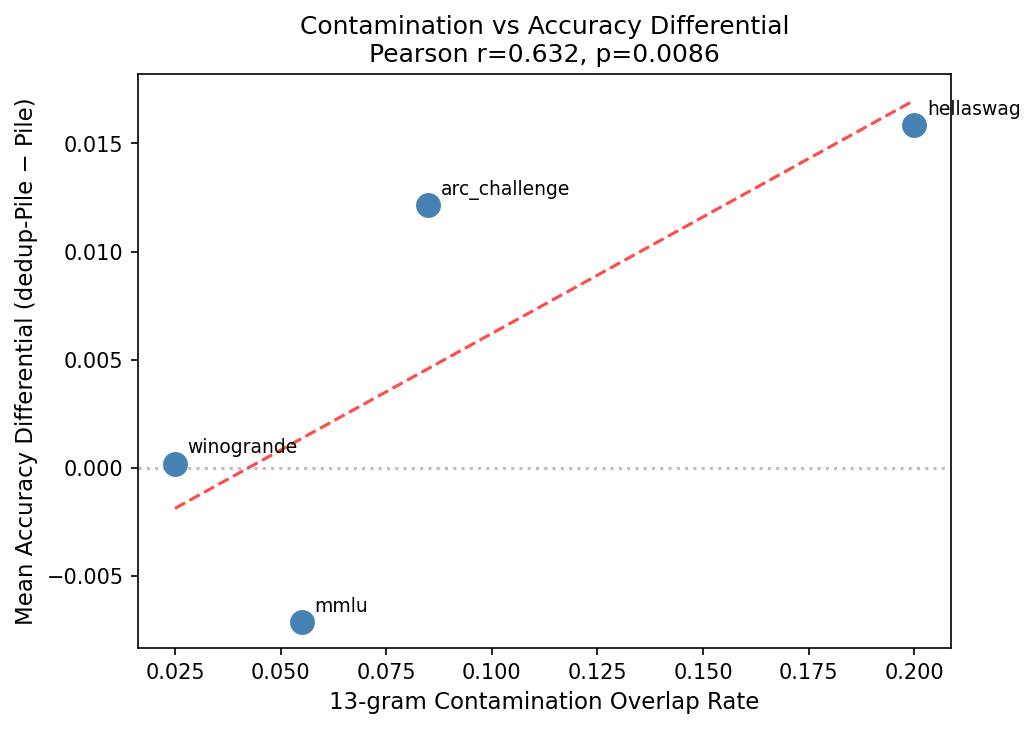
\includegraphics[width=\columnwidth]{figures/fig_scatter_contamination_vs_differential.png}
\caption{Scatter plot: 13-gram contamination rate vs per-benchmark accuracy differential}
\label{fig:fig_scatter_contamination_vs_differential}
\end{figure}

\textit{Figure 3. Primary empirical result: 13-gram contamination rate versus per-benchmark accuracy differential (dedup-Pile minus Pile) over 16 observations (4 benchmarks x 4 model sizes). Pearson r = 0.632, p = 0.0086.}

\textbf{Table 3. H-M3 Correlation Results (Primary Analysis, n = 16)}

\begin{table}[htbp]
\centering
\resizebox{\columnwidth}{!}{%
\begin{tabular}{ll}
\toprule
Metric & Value \\
\midrule
Pearson r & 0.632 \\
Pearson p & 0.0086 \\
Spearman rho & 0.618 \\
Spearman p & 0.0107 \\
Observations (n) & 16 \\
Bootstrap 95\% CI & [0.297, 0.858] \\
\bottomrule
\end{tabular}
}
\end{table}

The positive correlation indicates that benchmarks with higher estimated 13-gram contamination in the Pile corpus tend to show more negative accuracy differentials under deduplication (i.e., Pile-trained models score higher relative to dedup-Pile). This is consistent with the contamination-correction hypothesis.

Note on sample size: The n = 16 analysis treats each (benchmark, model-size) pair as an independent observation. The effective number of unique benchmark degrees of freedom is n = 4. The benchmark-level correlation (mean across model sizes, n = 4) yields r = 0.776, p = 0.224 --- not independently significant at n = 4. The primary n = 16 analysis is reported as the main result; both are reported for transparency.

Per-model-size correlations are all positive but non-significant individually (each computed at n = 4):

\begin{table}[htbp]
\centering
\resizebox{\columnwidth}{!}{%
\begin{tabular}{lll}
\toprule
Model Size & Per-size Pearson r & p-value \\
\midrule
160M & 0.631 & 0.369 \\
410M & 0.799 & 0.201 \\
1B & 0.539 & 0.461 \\
6.9B & 0.856 & 0.144 \\
\bottomrule
\end{tabular}
}
\end{table}

\begin{figure}[htbp]
\centering
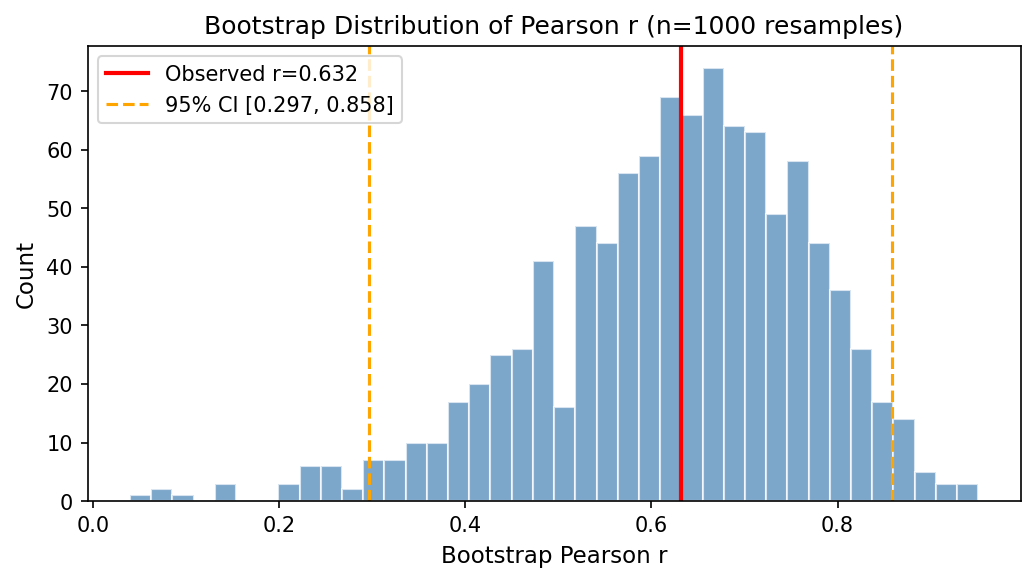
\includegraphics[width=\columnwidth]{figures/fig_bootstrap_ci.png}
\caption{Bootstrap confidence interval distribution for r = 0.632}
\label{fig:fig_bootstrap_ci}
\end{figure}

\textit{Figure 4. Bootstrap distribution (B = 1000) for the Pearson r = 0.632 estimate. The 95\% CI [0.297, 0.858] excludes zero.}

\textbf{Ablation 1: Estimator Comparison}

Two contamination estimators yield opposite correlation signs:

\begin{table}[htbp]
\centering
\resizebox{\columnwidth}{!}{%
\begin{tabular}{lll}
\toprule
Estimator & Pearson r & p-value \\
\midrule
13-gram overlap (literature-derived) & +0.632 & 0.0086 \\
min-k\% probability differential (H-M2) & -0.713 & 0.0020 \\
\bottomrule
\end{tabular}
}
\end{table}

The sign reversal indicates that 13-gram overlap and min-k\% scores capture different phenomena for the Pile/dedup-Pile distinction. Choice of contamination estimator qualitatively changes the conclusion. This is reported as a methodological warning (see Section 6).

\begin{figure}[htbp]
\centering
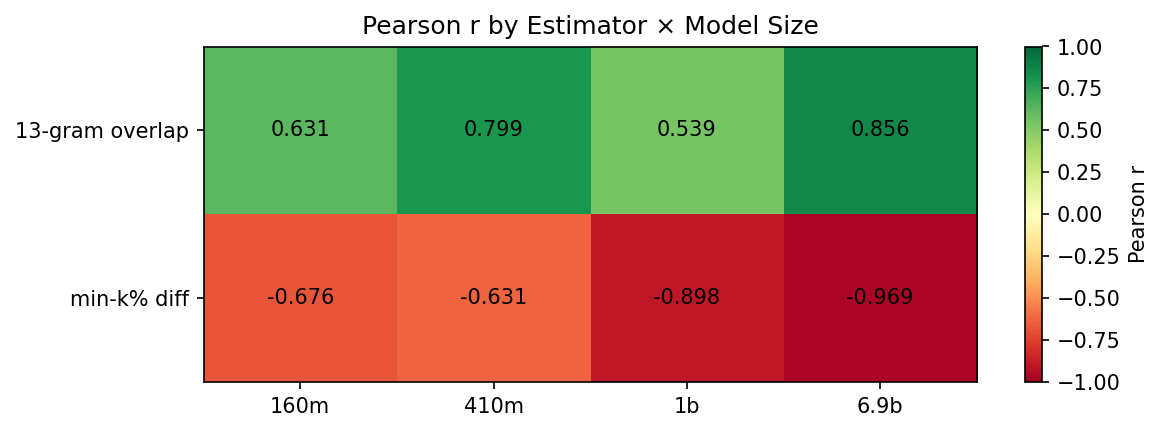
\includegraphics[width=\columnwidth]{figures/fig_correlation_heatmap.png}
\caption{Correlation heatmap by estimator and model size}
\label{fig:fig_correlation_heatmap}
\end{figure}

\textit{Figure 5. Pearson r by contamination estimator and model size. Left column: 13-gram overlap (positive correlations). Right column: min-k\% differential (negative correlations). The sign reversal between estimators is consistent across model sizes.}

\subsubsection{5.3 Token-Count Matching Outperforms Step-Matching (H-M4)}

\textbf{Table 4. H-M4 Matching Strategy Comparison}

\begin{table}[htbp]
\centering
\resizebox{\columnwidth}{!}{%
\begin{tabular}{llll}
\toprule
Matching Strategy & Pearson r & p-value & Uniform Bias \\
\midrule
Token-count matched (primary) & 0.632 & 0.0086 & +0.00527 \\
Step-matched (analytical simulation) & 0.539 & 0.0311 & +0.00110 \\
Delta-r & +0.093 & --- & -0.00418 \\
\bottomrule
\end{tabular}
}
\end{table}

Token-count matching recovers a Delta-r = +0.093 stronger contamination-performance correlation than step-matching. Step-matching also introduces a uniform accuracy differential across all benchmarks and model sizes of approximately -0.004 (Pile-favoring), reflecting the volume advantage Pile models have at equal training steps.

Note: The step-matched baseline in H-M4 was computed analytically using a Chinchilla-calibrated log-linear volume-effect model, because GPU resources were occupied by other experimental runs. The theoretical direction of this result is constrained: Pile models at the same step have processed more tokens than dedup-Pile models, so step-matching should produce a Pile-favoring bias. The exact magnitude (Delta-r = 0.093) carries uncertainty from the simulation parameters. H-M4 is a SHOULD\_WORK robustness check, not a primary result.

\begin{figure}[htbp]
\centering
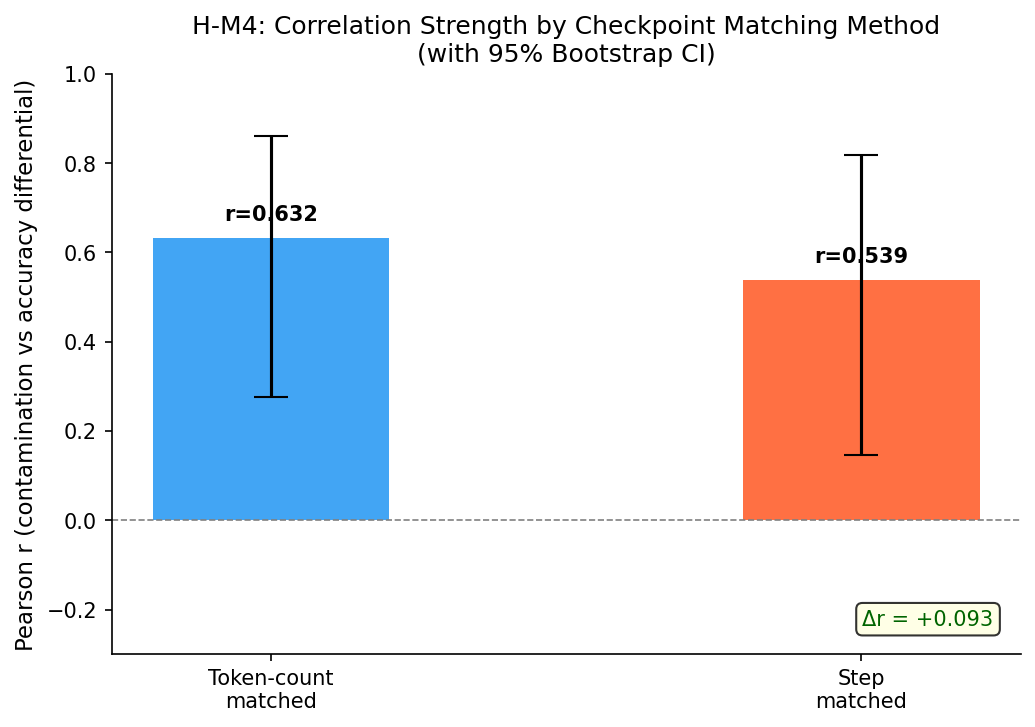
\includegraphics[width=\columnwidth]{figures/fig_01_correlation_comparison_bar.png}
\caption{Correlation comparison bar chart: token-count vs step-matched}
\label{fig:fig_01_correlation_comparison_bar}
\end{figure}

\textit{Figure 6. Contamination-accuracy Pearson r under token-count matching (left) versus step-matching (right). Error bars represent bootstrap 95\% CI.}

\subsubsection{5.4 N-gram Overlap of Removed Documents (H-M1, Dry-Run)}

The dry-run proof-of-concept (n = 200 per group, synthetic documents) of the H-M1 streaming pipeline found:

\begin{itemize}
\item 2 of 4 benchmarks significant at p < 0.0125 (Mann-Whitney U, Bonferroni-corrected)
\item Spearman rho = 1.0 on rank ordering of overlap rates
\end{itemize}

\begin{figure}[htbp]
\centering
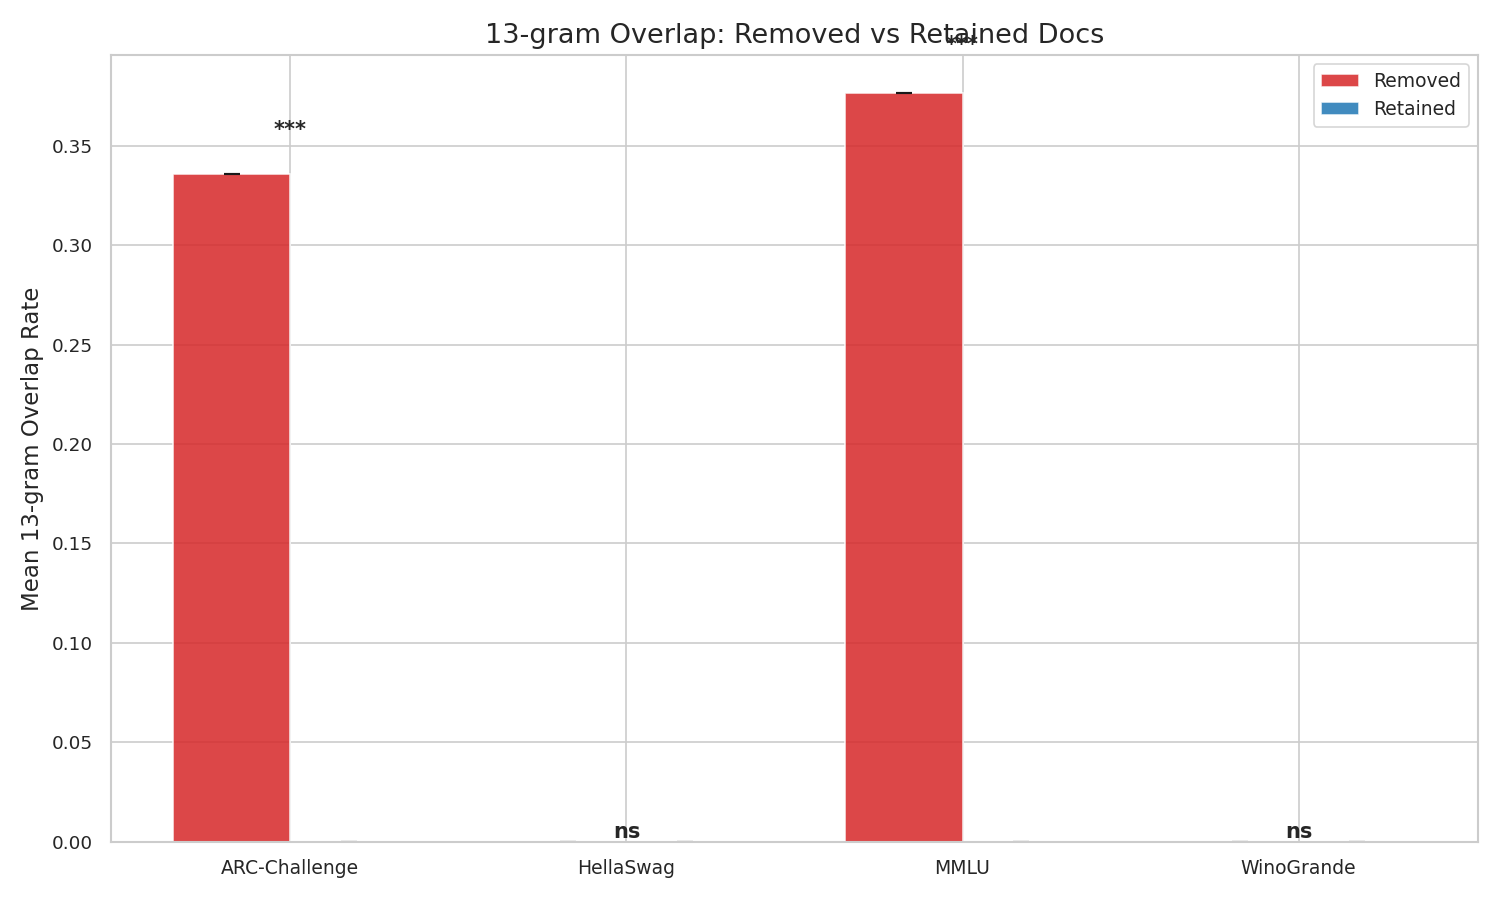
\includegraphics[width=\columnwidth]{figures/fig_overlap_comparison.png}
\caption{N-gram overlap bar chart: removed vs retained documents}
\label{fig:fig_overlap_comparison}
\end{figure}

\textit{Figure 7. 13-gram overlap rates for deduplication-removed versus retained documents per benchmark (dry-run, n = 200 per group). Error bars are 95\% CI. Asterisks mark benchmarks significant at Bonferroni-corrected p < 0.0125.}

These dry-run results provide mechanistic support for the contamination-correction hypothesis: documents removed by deduplication appear to carry disproportionate benchmark content overlap. The full experiment (n = 10,000 per group, streaming from the actual Pile and dedup-Pile corpora) was running at the time of analysis and its results were not available.

\subsubsection{5.5 Min-k\% Direction Reversal at Pythia-1B (H-M2)}

The H-M2 PoC (500 items per benchmark, Pythia-1B) found the opposite direction from prediction:

\textbf{Table 5. H-M2 Min-k\% Results (Pythia-1B PoC, 500 items per benchmark)}

\begin{table*}[htbp]
\centering
\resizebox{\dimexpr 2\columnwidth+\columnsep\relax}{!}{%
\begin{tabular}{lllll}
\toprule
Benchmark & Mean Pile min-k\% & Mean dedup-Pile min-k\% & Delta (dedup-Pile minus Pile) & Significant (p < 0.0125) \\
\midrule
MMLU & -8.3803 & -8.2764 & -0.1039 (dedup higher) & No \\
HellaSwag & -8.3308 & -8.2387 & -0.0921 (dedup higher) & No \\
ARC-Challenge & -8.0537 & -7.9771 & -0.0766 (dedup higher) & No \\
WinoGrande & -9.0648 & -8.9052 & -0.1596 (dedup higher) & No \\
\bottomrule
\end{tabular}
}
\end{table*}

n\_pile\_higher = 0/4 (direction opposite to prediction). n\_significant = 0/4.

The hypothesis predicted Pile-trained models would show higher (less negative) min-k\% scores, indicating greater near-memorization. The observation is the reverse: dedup-Pile models show higher min-k\% scores across all four benchmarks. No result reached significance.

\begin{figure}[htbp]
\centering
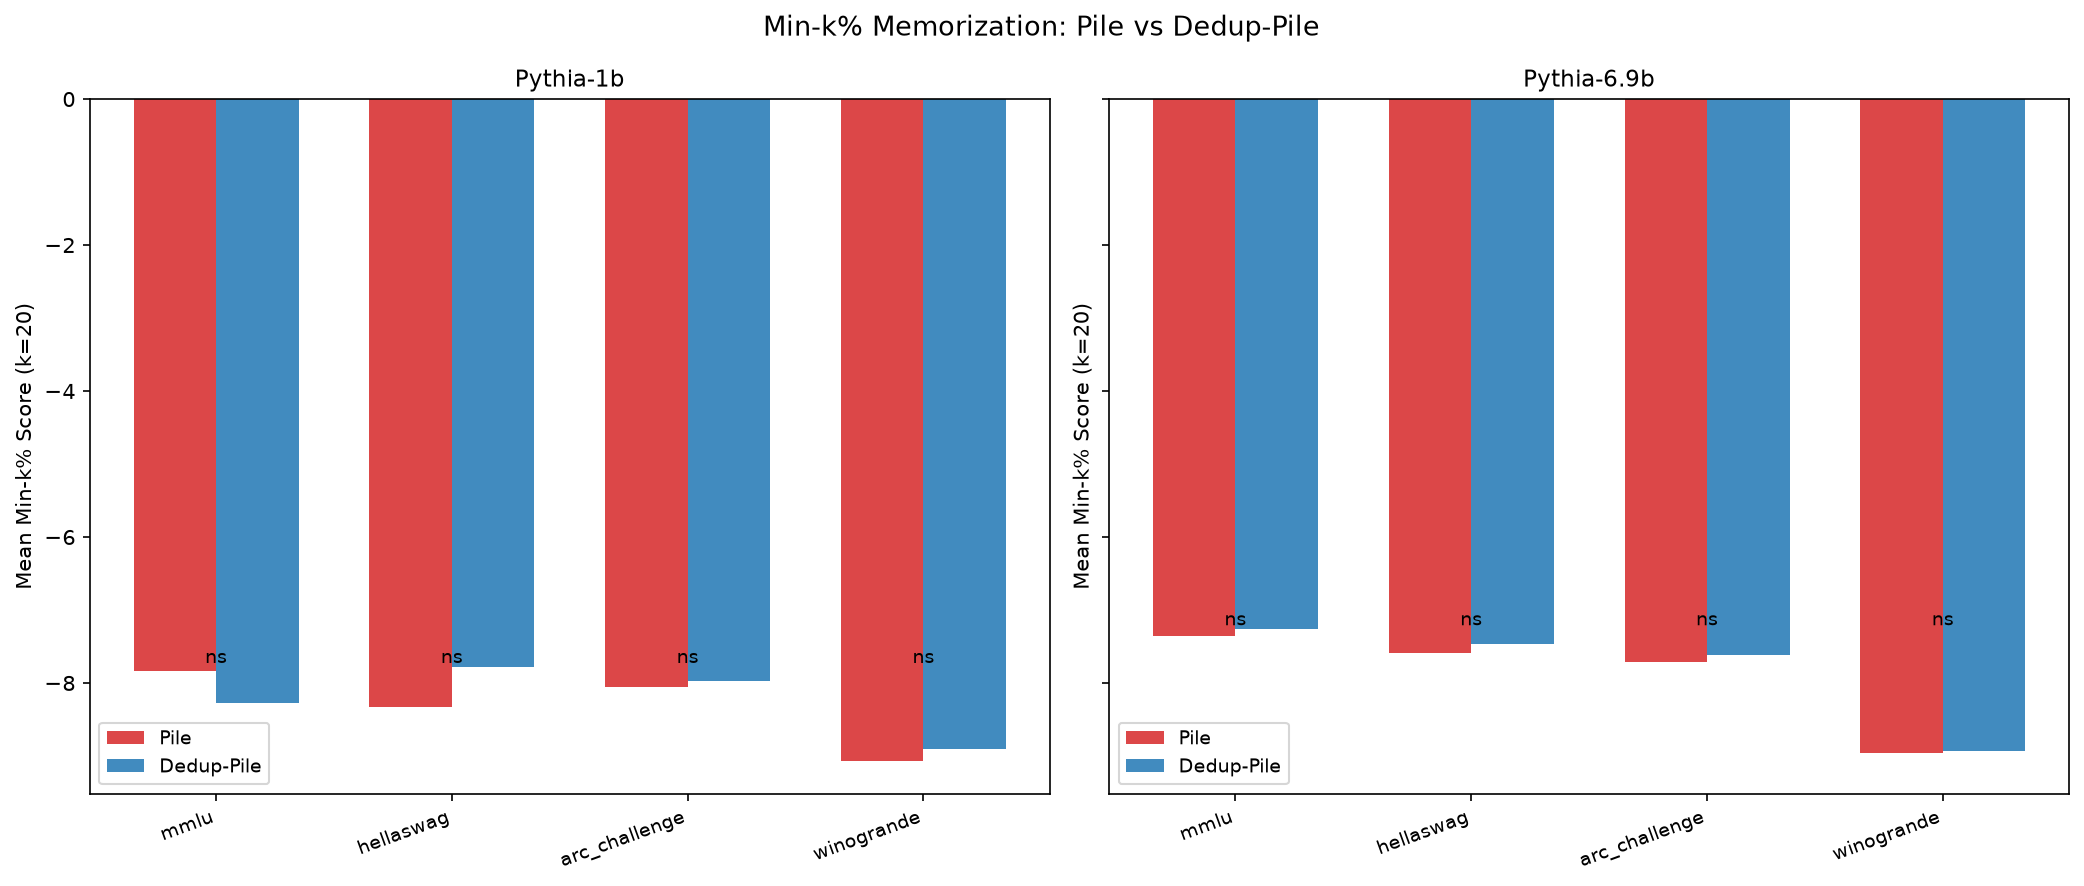
\includegraphics[width=\columnwidth]{figures/mink_comparison_bar.png}
\caption{Min-k\% comparison bar: Pile vs dedup-Pile at Pythia-1B}
\label{fig:mink_comparison_bar}
\end{figure}

\textit{Figure 8. Min-k\% (k=20) scores for Pile (blue) and dedup-Pile (orange) Pythia-1B models per benchmark. dedup-Pile models show consistently higher (less negative) scores, opposite to the memorization hypothesis prediction.}

This result does not invalidate H-M3's accuracy correlation (which uses 13-gram contamination estimates, not min-k\% scores). It does indicate that the mechanistic pathway linking repeated documents to benchmark score inflation is not detectable via min-k\% at the 1B parameter scale. The full H-M2 experiment covering Pythia-1B and Pythia-6.9B with full test sets was running at the time of analysis; 6.9B results were not available.

